\section{Resultados}


\begin{frame}[c]{DeepLabV3}{Com backbone Resnet50}

    \begin{columns}
      \column{0.4\textwidth}
            \begin{itemize}
                  \item 41M de parâmetros
                  \item 17M treinaveis
            \end{itemize}
      \column{0.5\textwidth}
            \begin{itemize}
                  \item Não houve convergência
                  \item Complicações com o treino
            \end{itemize}
    \end{columns}

    
  \end{frame}


\begin{frame}[c]{U-net}{Treinada do raíz}

  \begin{columns}

    \column{0.5\textwidth}
      \begin{itemize}
            \item 33M de parâmetros
            \item 33M treinaveis
      \end{itemize}

    \column{0.5\textwidth}
    \begin{itemize}
      \item Exatidão de 76\% \\Época 157
    \end{itemize}


  \end{columns}

\end{frame}

\newcommand{\plotA}{\inserttrainvalplot{resources/data/train_info_unet_200_smooth.csv}{ylabel=Loss, xmin=0, xmax=157, ymin=0, ymax=2, title=U-Net from scratch - Smoothed losses}{Train losses}{Validation losses}{north east}}
\newcommand{\plotB}{\inserttrainvalplot{resources/data/train_info_unet_200_smooth.csv}{ylabel=DICE Score, xmin=0, xmax=157, ymin=0, ymax=1, title=U-Net from scratch - Smoothed DICE scores}{Train DICE}{Validation DICE}{north west}}

\begin{frame}[c]{U-net}{Treinada do raíz}

    \begin{figure}[ht]
        \centering
        \only<1>\plotA
        \only<2>\plotB
    \end{figure}

\end{frame}


\begin{frame}[c]{U-net}{Com Resnet50 Backbone}

    \begin{columns}

        \column{0.5\textwidth}
          \begin{itemize}
                \item 148M de parâmetros
                \item 124M treinaveis
          \end{itemize}
    
        \column{0.5\textwidth}
        \begin{itemize}
          \item Exatidão de 85\% \\Época 142
        \end{itemize}
    
    
      \end{columns}
    
  \end{frame}

\newcommand{\plotC}{\inserttrainvalplot{resources/data/train_info_resnet_frozzen_200_smooth.csv}{ylabel=Loss, xmin=0, xmax=142, ymin=0, ymax=2, title=U-Net with ResNet50 (frozen) - Smoothed losses}{Train losses}{Validation losses}{north east}}
\newcommand{\plotD}{\inserttrainvalplot{resources/data/train_info_resnet_frozzen_200_smooth.csv}{ylabel=DICE Score, xmin=0, xmax=142, ymin=0, ymax=1, title=U-Net with ResNet50 (frozen) - Smoothed DICE scores}{Train DICE}{Validation DICE}{south east}}

\begin{frame}[c]{U-net}{Com Resnet50 Backbone}
\begin{figure}[ht]
    \centering
    \only<1>\plotC
    \only<2>\plotD
\end{figure}

\end{frame}


  \begin{frame}[c]{U-net}{Com Resnet50 Backbone}

    \begin{columns}

        \column{0.5\textwidth}
          \begin{itemize}
                \item 148M de parâmetros
                \item 148M treinaveis
          \end{itemize}
    
        \column{0.5\textwidth}
        \begin{itemize}
          \item Exatidão de 85\% \\Época 17
        \end{itemize}
    
    
      \end{columns}
    
  \end{frame}
\newcommand{\plotone}{\inserttrainvalplot{resources/data/train_info_resnet_unfrozzen_200_smooth.csv}{ylabel=Loss, xmin=0, xmax=17, ymin=0, ymax=2, title=U-Net with ResNet50 (unfrozen) - Smoothed losses}{Train losses}{Validation losses}{north east}}
\newcommand{\plottwo}{\inserttrainvalplot{resources/data/train_info_resnet_unfrozzen_200_smooth.csv}{ylabel=DICE Score, xmin=0, xmax=17, ymin=0, ymax=1, title=U-Net with ResNet50 (unfrozen) - Smoothed DICE scores}{Train DICE}{Validation DICE}{south east}}
  \begin{frame}[c, fragile]{U-net}{Com Resnet50 Backbone}
    \begin{figure}[ht]
        \centering
        % \only<1>\inserttrainvalplot{resources/data/train_info_resnet_unfrozzen_200_smooth.csv}{ylabel=Loss, xmin=0, xmax=17, ymin=0, ymax=2, title=U-Net with ResNet50 (unfrozen) - Smoothed losses}{Train losses}{Validation losses}{north east}
        % \only<2>\inserttrainvalplot{resources/data/train_info_resnet_unfrozzen_200_smooth.csv}{ylabel=DICE Score, xmin=0, xmax=17, ymin=0, ymax=1, title=U-Net with ResNet50 (unfrozen) - Smoothed DICE scores}{Train DICE}{Validation DICE}{south east}
        \only<1>\plotone
        \only<2>\plottwo
        
    \end{figure}

  \end{frame}


\begin{frame}[c]{Alguns resultados do melhor modelo}
    \begin{figure}[ht]
        \centering
        \begin{minipage}[b]{0.45\linewidth}
            \centering
            \only<1>{\includegraphics[width=1\textwidth]{resources/images/gtruth/pattern_58.jpg}}
            \only<2>{\includegraphics[width=1\textwidth]{resources/images/gtruth/pattern_61.jpg}}
            \only<3>{\includegraphics[width=1\textwidth]{resources/images/gtruth/pattern_63.jpg}}
            \only<4>{\includegraphics[width=1\textwidth]{resources/images/gtruth/rgbd_hand_color_190.jpg}}
            \captionsetup{labelformat=empty}
            \caption{Resultado esperado}
        \end{minipage}
        \hspace{0.5cm}
        \begin{minipage}[b]{0.45\linewidth}
            \centering
            \only<1>{\includegraphics[width=1\textwidth]{resources/images/preds/Small_dataset_unet_resnet/pattern_58.jpg}}
            \only<2>{\includegraphics[width=1\textwidth]{resources/images/preds/Small_dataset_unet_resnet/pattern_61.jpg}}
            \only<3>{\includegraphics[width=1\textwidth]{resources/images/preds/Small_dataset_unet_resnet/pattern_63.jpg}}
            \only<4>{\includegraphics[width=1\textwidth]{resources/images/preds/Small_dataset_unet_resnet/rgbd_hand_color_190.jpg}}
            \captionsetup{labelformat=empty}
            \caption{Resultado obtido}
        \end{minipage}
    \end{figure}
\end{frame}
